\documentclass[11pt,fleqn]{article}

\setlength {\topmargin} {-.15in}
\setlength {\textheight} {8.6in}

\usepackage{amsmath}
\usepackage{amssymb}
\usepackage{color}
\usepackage{tikz}
\usetikzlibrary{automata,positioning,arrows}
\usepackage{diagbox}
\usepackage{stackrel}

\renewcommand{\labelenumi}{\theenumi.}
\renewcommand{\labelenumii}{\theenumii.}
\renewcommand{\labelenumiii}{\theenumiii.}
\newcommand{\be}{\begin{enumerate}}
	\newcommand{\ee}{\end{enumerate}}
\newcommand{\bi}{\begin{itemize}}
	\newcommand{\ei}{\end{itemize}}
\newcommand{\bc}{\begin{center}}
	\newcommand{\ec}{\end{center}}
\newcommand{\bsp}{\begin{sloppypar}}
	\newcommand{\esp}{\end{sloppypar}}
\newcommand{\mname}[1]{\mbox{\sf #1}}
\newcommand{\sB}{\mbox{$\cal B$}}
\newcommand{\sC}{\mbox{$\cal C$}}
\newcommand{\sF}{\mbox{$\cal F$}}
\newcommand{\sM}{\mbox{$\cal M$}}
\newcommand{\sP}{\mbox{$\cal P$}}
\newcommand{\sV}{\mbox{$\cal V$}}
\newcommand{\set}[1]{{\{ #1 \}}}
\newcommand{\Neg}{\neg} 
\ifdefined \And 
\renewcommand{\And}{\wedge}
\else
\newcommand{\And}{\wedge}
\fi
\newcommand{\Or}{\vee}
\newcommand{\Implies}{\Rightarrow}
\newcommand{\Iff}{\Leftrightarrow}
\newcommand{\Forall}{\forall}
\newcommand{\ForallApp}{\forall\,}
\newcommand{\Forsome}{\exists}
\newcommand{\ForsomeApp}{\exists\,}
\newcommand{\mdot}{\mathrel.}
\newcommand{\der}[2]{\stackrel[#2]{#1}{\longrightarrow}}
\newcommand{\nt}[1]{\seq{\texttt{#1}}}
\newcommand{\seq}[1]{{\langle #1 \rangle}}
\newcommand{\sglsp}{\ }
\newcommand{\dblsp}{\ \ }
\newenvironment{proof}{\par\noindent{\bf Proof\sglsp}}{\hfill$\Box$}
\newcommand{\pnote}[1]{{\langle \text{#1} \rangle}}

\begin{document}
	
	\begin{center}
		
		{\large \textbf{COMPSCI/SFWRENG 2FA3}}\\[2mm]
		{\large \textbf{Discrete Mathematics with Applications II}}\\[2mm]
		{\large \textbf{Winter 2021}}\\[8mm]
		{\huge \textbf{Assignment 8 with Solutions}}\\[6mm]
		{\large \textbf{Dr.~William M. Farmer and Dr.~Mehrnoosh Askarpour}}\\[2mm]
		{\large \textbf{McMaster University}}\\[6mm]
		{\large Revised: March 28, 2021}
		
	\end{center}
	
	\medskip
	
	Assignment 8 consists of two problems.  You must write your solutions
	to the problems using LaTeX.
	
	Please submit Assignment~8 as two files,
	\texttt{Assignment\_8\_\emph{YourMacID}.tex} and
	\texttt{Assignment\_8\_\emph{YourMacID}.pdf}, to the Assignment~8
	folder on Avenue under Assessments/Assignments.
	\texttt{\emph{YourMacID}} must be your personal MacID (written without
	capitalization).  The \texttt{Assignment\_8\_\emph{YourMacID}.tex}
	file is a copy of the LaTeX source file for this assignment
	(\texttt{Assignment\_8.tex} found on Avenue under
	Contents/Assignments) with your solution entered after each problem.
	The \texttt{Assignment\_8\_\emph{YourMacID}.pdf} is the PDF output
	produced by executing
	
	\begin{itemize}
		
		\item[] \texttt{pdflatex Assignment\_8\_\emph{YourMacID}}
		
	\end{itemize}
	
	This assignment is due \textbf{Sunday, March 28, 2021 before
		midnight.}  You are allow to submit the assignment multiple times,
	but only the last submission will be marked.  \textbf{Late submissions
		and files that are not named exactly as specified above will not be
		accepted!}  It is suggested that you submit your preliminary
	\texttt{Assignment\_8\_\emph{YourMacID}.tex} and
	\texttt{Assignment\_8\_\emph{YourMacID}.pdf} files well before the
	deadline so that your mark is not zero if, e.g., your computer fails
	at 11:50 PM on March 28.
	
	\textbf{Although you are allowed to receive help from the
		instructional staff and other students, your submission must be your
		own work.  Copying will be treated as academic dishonesty! If any of
		the ideas used in your submission were obtained from other students
		or sources outside of the lectures and tutorials, you must
		acknowledge where or from whom these ideas were obtained.}
	
	\newpage
	
	\subsection*{Problems}
	
	\be
	
	\item  Construct PDAs for the languages below. For each language, if it is deterministic CFL, then define a DPDA, otherwise an NPDA.
	\be
	\item\textbf{[5 points]} $L = \{a^nb^m \mid 1 \le n \le m \}
$
	\item\textbf{[5 points]} $L = \{a^nb^m \mid 1 \le n < m \}$
	\item\textbf{[5 points]} $L = \{a^nb^m \mid 1 \le m \le n \}$
	\item\textbf{[5 points]} $L = \{a^nb^m \mid 1 \le m < n \}$ 
	\ee

	\ee
	\textbf{Aamina Hussain, hussaa54, March 28, 2021}\\
	
	\noindent\textbf{\emph{Part A:}}\\
	Let $M = (Q, \Sigma, \Gamma, \delta, s, \bot, F)$ represent the PDA defined below where:\\
	$Q = \set{q_0, q_1, q_2}$\\
	$\Sigma = \set{a, b}$\\
	$\Gamma = \set{\bot, A}$\\
	$s = q_0$\\
	$F = \set{q_2}$

	\noindent$\delta$ contains the following transitions:
	\be
	\item $((q_0, a, \bot),\ (q_1, A\bot))$
	\item $((q_1, a, A),\ (q_1, AA))$
	\item $((q_1, b, A),\ (q_1, \epsilon))$
	\item $((q_1, b, \bot),\ (q_1, \bot))$
	\item $((q_1, \epsilon, \bot),\ (q_2, \bot))$
	\ee

	\begin{center}
	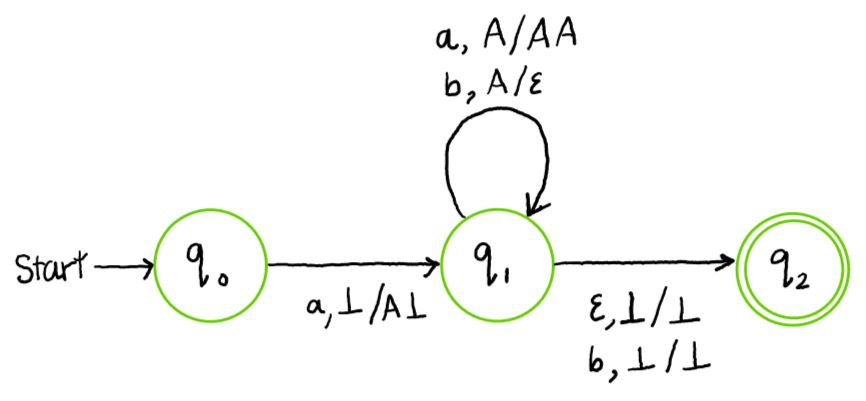
\includegraphics[scale = 0.5]{A8partA.JPG}
	\end{center}
	
	\noindent\textbf{\emph{Part B:}}\\
	Let $M = (Q, \Sigma, \Gamma, \delta, s, \bot, F)$ represent the PDA defined below where:\\
	$Q = \set{q_0, q_1, q_2, q_3}$\\
	$\Sigma = \set{a, b}$\\
	$\Gamma = \set{\bot, A}$\\
	$s = q_0$\\
	$F = \set{q_3}$

	\noindent$\delta$ contains the following transitions:
	\be
	\item $((q_0, a, \bot),\ (q_1, A\bot))$
	\item $((q_1, a, A),\ (q_1, AA))$
	\item $((q_1, b, A),\ (q_1, \epsilon))$
	\item $((q_1, b, \bot),\ (q_1, \bot))$
	\item $((q_1, b, \bot),\ (q_2, \bot))$
	\item $((q_2, \epsilon, \bot),\ (q_3, \bot))$
	\ee

	\begin{center}
	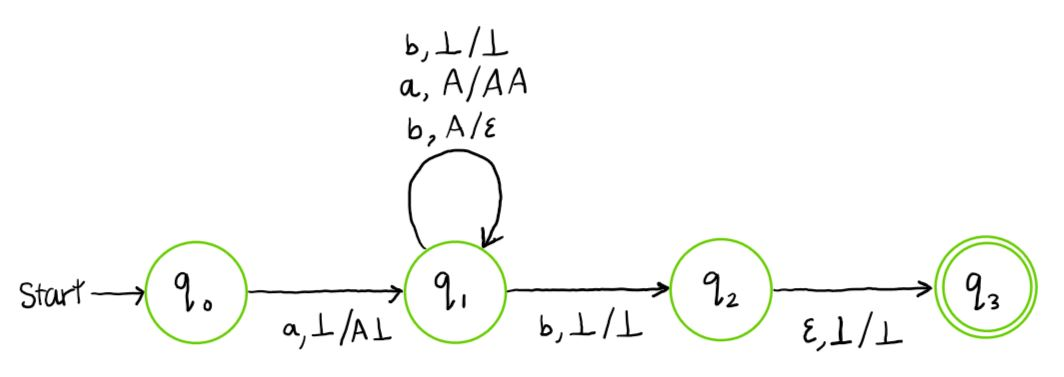
\includegraphics[scale = 0.5]{A8partB.JPG}
	\end{center}

	\noindent\textbf{\emph{Part C:}}\\
	Let $M = (Q, \Sigma, \Gamma, \delta, s, \bot, F)$ represent the PDA defined below where:\\
	$Q = \set{q_0, q_1, q_2, q_3}$\\
	$\Sigma = \set{a, b}$\\
	$\Gamma = \set{\bot, A}$\\
	$s = q_0$\\
	$F = \set{q_3}$

	\noindent$\delta$ contains the following transitions:
	\be
	\item $((q_0, a, \bot),\ (q_1, A\bot))$
	\item $((q_1, a, A),\ (q_1, AA))$
	\item $((q_1, b, A),\ (q_2, \epsilon))$
	\item $((q_2, b, A),\ (q_2, \epsilon))$
	\item $((q_2, \epsilon, A),\ (q_3, A))$
	\item $((q_2, \epsilon, \bot),\ (q_3, \bot))$
	\ee

	\begin{center}
	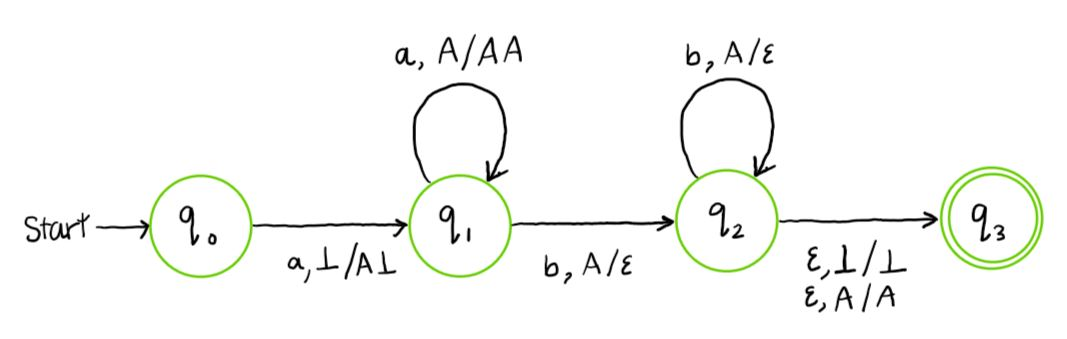
\includegraphics[scale = 0.5]{A8partC.JPG}
	\end{center}

	\noindent\textbf{\emph{Part D:}}\\
	Let $M = (Q, \Sigma, \Gamma, \delta, s, \bot, F)$ represent the PDA defined below where:\\
	$Q = \set{q_0, q_1, q_2, q_3}$\\
	$\Sigma = \set{a, b}$\\
	$\Gamma = \set{\bot, A}$\\
	$s = q_0$\\
	$F = \set{q_3}$

	\noindent$\delta$ contains the following transitions:
	\be
	\item $((q_0, a, \bot),\ (q_1, A\bot))$
	\item $((q_1, a, A),\ (q_1, AA))$
	\item $((q_1, b, A),\ (q_2, \epsilon))$
	\item $((q_2, b, A),\ (q_2, \epsilon))$
	\item $((q_2, \epsilon, A),\ (q_3, A))$
	\ee
	
	\begin{center}
	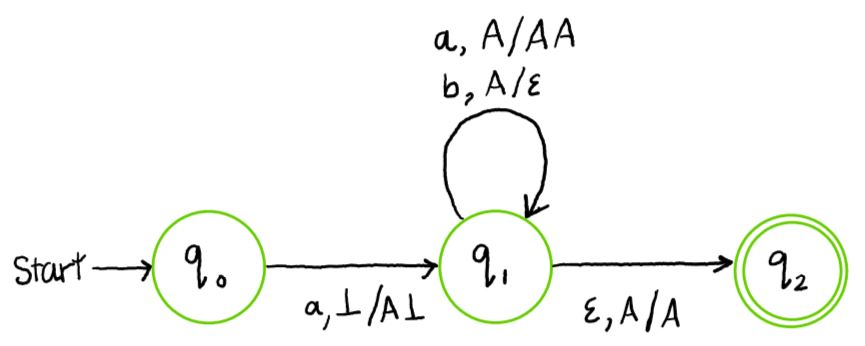
\includegraphics[scale = 0.5]{A8partD.JPG}
	\end{center}

	
	
\end{document}


